% !TeX spellcheck = en_GB

\section{Requirements}\label{sec:requirements}

The following sections describe the primary requirements in the form of user stories~\cite{agile-alliance-user-stories}.
Figure \ref{fig:requirements-overview} shows an overview of the primary use stories.

\begin{figure}[h]
    \centering
    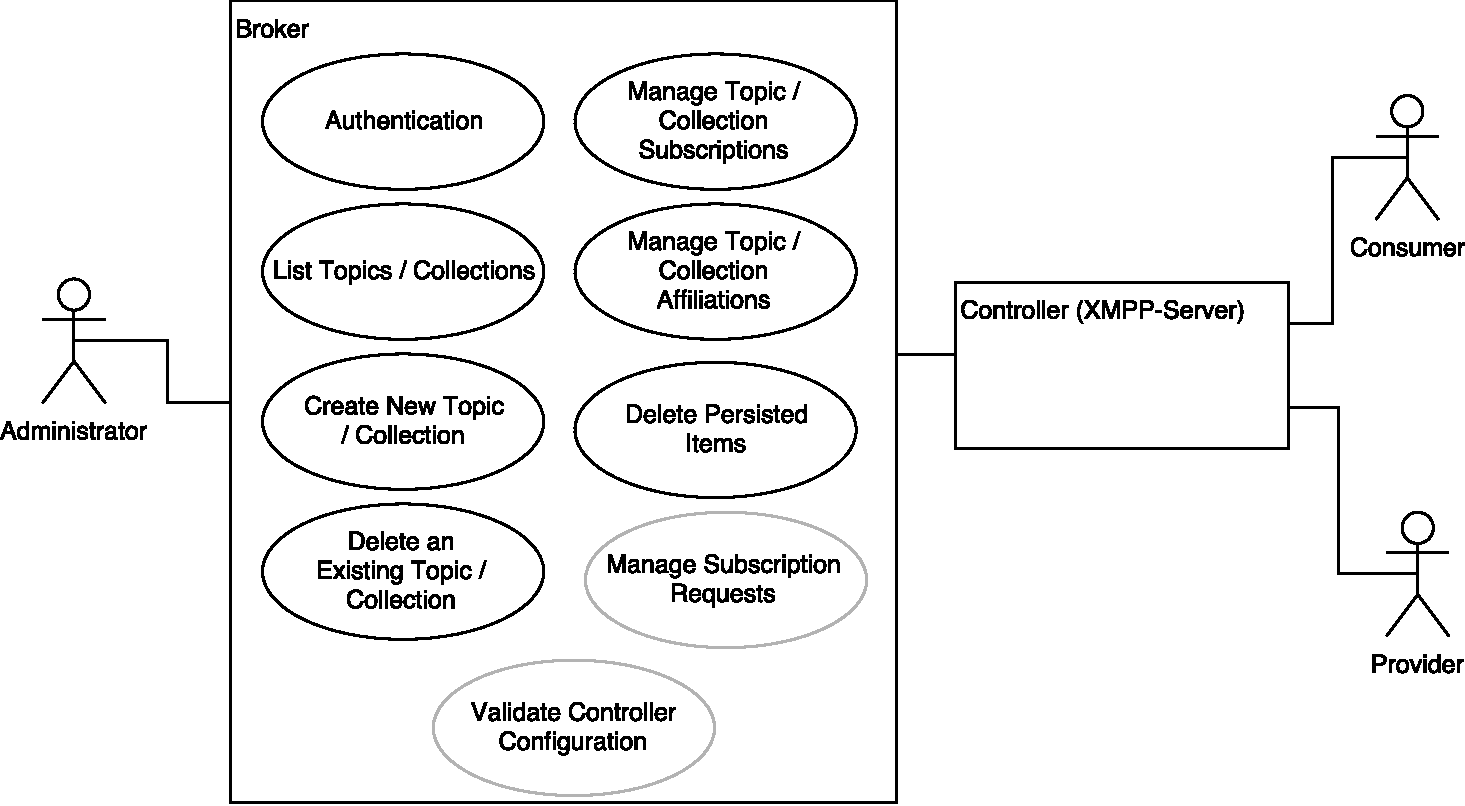
\includegraphics[width=1\linewidth]{resources/requirements_overview}
    \caption{UML Use Case Diagram presenting an overview of the primary user stories.}
    \label{fig:requirements-overview}
\end{figure}

\noindent\textcolor{red}{To be clarified}

\begin{itemize}
    \item Non Functional Requirements
\end{itemize}


\subsection{Authentication}
\subsubsection{Login}

As an Administrator,\\
I want to log in\\
- preferably using an existing client TLS certificate - \\
so that only I can inspect and manage Topics.\\

\subsubsection{Secure XMPP Authentication}

As an Administrator concerned with security requirements,\\
I want to use either SASL EXTERNAL or SASL SCRAM mechanism for authentication -

\begin{itemize}
    \item preferably the SCRAM-SHA-256-PLUS variant and
    \item preferably using mutual certificate-based authentication including revocation status checking
\end{itemize}

\noindent - so that the Controller is fully compatible with the XMPP grid draft~\cite{ietf-mile-xmpp-grid-05}.

\noindent To achieve this goal, I am willing to accept:
\begin{itemize}
    \item More costly and less user friendly authentication
    \item limited compatibility of supported XMPP servers
\end{itemize}

\subsubsection{Secure XMPP Connection}

As an Administrator concerned with security requirements,\\
I want to use minimally TLS 1.2 [RFC5246] to communicate with the XMPP server at all times\\
to achieve maximal security and compatibility with the XMPP grid draft~\cite{ietf-mile-xmpp-grid-05}.

\subsubsection{Secure Connection}

As an Administrator concerned with security requirements,\\
I want to use minimally TLS 1.2 [RFC5246] to communicate with the Broker\\
to achieve maximal security.

\subsubsection{Multiple Administrations}

As an Administrator,\\
I want to grant access to administrators \\
so that they can also manage the application.

\subsubsection{Audit Trail}

As an Administrator concerned with security requirements,\\
I want to be able to access an audit log\\
- preferably using existing XMPP mechanisms - \\
so that I can reconstruct what other Administrations did on the Controller.

\subsubsection{Logout}

As an Administrator,\\
I want to log out\\
so that I can terminate a session.

\subsection{List Topics}

\subsubsection{List All Topics}
As an Administrator,\\
I want to see a list of all Topics of the associated Controller\\
so that I can quickly assimilate which Topics exist.

\noindent\textcolor{red}{To be clarified}

\begin{itemize}
    \item How many topics are realistic? 1-10, 10-100, 100-1000, > 1000? (search required?)
\end{itemize}


\subsubsection{List Available Topics With Limited Access}

As an Administrator,\\
I want to see a list of all Topics of the associated Controller to which I have limited access to,\\
to simplify troubleshooting and locate errors.

\noindent\textcolor{red}{\\To be clarified}

\begin{itemize}
    \item Is this a relevant scenario?
\end{itemize}


\subsection{Create a New Topic}

As an Administrator,\\
I want to create a new Topic on the associated Controller\\
so that I am not tied to a fixed set of Topics.

\subsubsection{Override Default Topic Configuration}

As an Administrator in the process of creating a new Topic,\\
I want to override the default configuration (e.g. the affiliations) \\
so that I can restrict access and provide reasonable defaults.

\subsubsection{Initial Topic Consumers and Providers}

As an Administrator in the process of creating a new Topic,\\
I want to specify an initial set of Consumers and Providers \\
so that I can restrict access to that Topic and provide reasonable defaults.

\subsection{Delete an Existing Topic}

As an Administrator,\\
I want to delete an existing Topic on the associated Controller\\
so that I can get rid of obsolete Topics.

\subsubsection{Fault Prevention On Delete}

As an Administrator in the process of deleting a Topic, \\
I want a mechanism to prevent me from deleting the wrong Topic on the associated Controller\\
(e.g. require me to enter the name of the Topic manually).

\subsection{Manage Topic Subscriptions}

\subsubsection{List Consumers}

As an Administrator, \\
I want to list all Consumers (including their JIDs) of a given Topic on the associated Controller, \\
so that I can verify that specific Consumers are subscribed, and others are not.

\noindent\textcolor{red}{To be clarified}

\begin{itemize}
    \item How many Consumers are realistic? 1-10, 10-100, 100-1000, > 1000? (search required?)
\end{itemize}


\subsubsection{Inspect Detailed Subscription Configuration}

As an Administrator, \\
I want to inspect the detailed Topic subscription configuration of a given Consumer, \\
so that I can reproduce and reason about the receipt of data on that Consumer
and find potential misconfiguration.

\subsubsection{Partially Modify Subscription Configuration}

As an Administrator, \\
I want to modify parts of the Topic subscription configuration of a given Consumers, \\
so that I can fix misconfiguration.

\subsubsection{Unsubscribe Consumer}

As an Administrator, \\
I want to manually unsubscribe a specific Consumer from a particular Topic on the associated Controller, \\
so that I can remove obsolete or undesired subscriptions.

\subsubsection{Subscribe Consumer}

As an Administrator, \\
I want to manually subscribe a specific Consumer on a particular Topic on the associated Controller, \\
so that I can faster setup and manage Consumers.

\subsection{Manage Topic Affiliations}
\subsubsection{Inspect Affiliations}

As an Administrator,\\
I want to list all Affiliations (JID and "Role") for a particular Topic on the associated Controller \\
so that I can find potential misconfiguration.

\noindent\textcolor{red}{To be clarified}

\begin{itemize}
    \item How many Consumers/Publishers are realistic?
\end{itemize}


\subsubsection{Modify Affiliations}

As an Administrator,\\
I want to modify the Affiliation ("Role") of a given JID for a particular Topic on the associated Controller \\
so that I can fix potential misconfiguration.

\subsubsection{Fault Prevention When Modifying My Affiliation}

As an Administrator in the process of modifying my Affiliation for a particular Topic on the associated Controller,\\
I want a mechanism to prevent me from accidentally downgrading my rights.

\subsubsection{Meaningful Error For Topics With Limited Access}

As an Administrator,\\
I want to receive a meaningful error message when inspecting a node to which I have limited access \\
so that I can quickly comprehend why the configuration options are limited.

\subsection{Manage Subscription Requests}

\subsubsection{List Subscription Request}
As an Administrator,\\
I want to list pending subscription requests for a given Topic\\
- given that this feature is supported by the associated Controller -\\
so that I can quickly assimilate pending requests.

\subsubsection{Accept Subscription Request}

As an Administrator,\\
I want to accept a pending subscription request for a given Topic\\
- given that this feature is supported by the associated Controller -\\
to enable more dynamic access models than just maintaining a black- or whitelist.

\subsubsection{Reject Subscription Request}

As an Administrator,\\
I want to reject a pending subscription request for a given Topic\\
- given that this feature is supported by the associated Controller -\\
so that I can deny user access in accordance with the XMPP standards.

\subsection{Delete Persisted Items From a Topic}

\subsubsection{Delete a Persisted Item From a Topic}

As an Administrator,\\
I want to delete a particular persisted item from a specific Topic\\
- given that this feature is supported by the associated Controller -\\
so that I can clean up test items and remove obsolete or corrupted items.

\subsubsection{Purge All Persisted Items From a Topic}

As an Administrator,\\
I want to purge persisted items from a specific Topic\\
- given that this feature is supported by the associated Controller -\\
so that I can clean up test items and remove obsolete or corrupted items.

\subsection{Validate Controller Configuration}

\subsubsection{Validate Supported XEPs Configurations}
As an Administrator,\\
I want to validate that a minimum set of XEPs are supported by the associated Controller\\
so that I can quickly identify incompatibilities.

\subsubsection{Validate Optional XEP Implementations}
As an Administrator,\\
I want to validate that the required features that are marked as optional or recommended in the XEPs are implemented by the associated Controller\\
so that I can quickly identify incompatibilities.

